% \documentclass[svgnames]{article}
% To make png: pdftopng -r 900 -alpha LucasBoston.pdf temp.png
\documentclass[svgnames,convert={density=900,size=720x600,outext=.png}]{standalone}
\usepackage{tikz}
\usetikzlibrary{calc,trees,positioning,arrows,chains,shapes.geometric,backgrounds,
  decorations.pathreplacing,decorations.pathmorphing,shapes,snakes,automata,
  matrix,shapes.symbols,mindmap,shadows,petri}
% \renewcommand{\rmdefault}{phv} % Arial
% \renewcommand{\sfdefault}{phv} % Arial
% \usepackage{amsmath} % to allow Sans font in math


\begin{document}
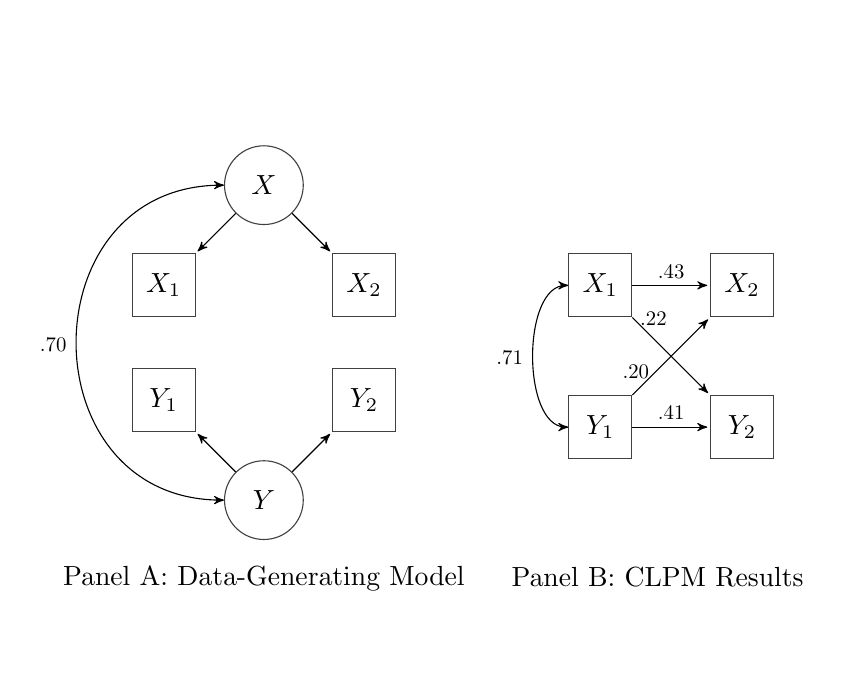
\begin{tikzpicture}[node distance=1.8cm,>=stealth',bend angle=45,auto]
  \useasboundingbox (-3,-6) rectangle (7,2);
  \tikzset{
    latentTrait/.style={ellipse,draw=black!75,minimum size=10mm, align=center},
    latentAR/.style={ellipse,draw=black!75,minimum size=7mm},
    observed/.style={rectangle,draw=black!75,minimum size=8mm, align=center},
    error/.style={circle,draw=black!75,minimum size=.9mm},
    errorAR/.style={circle,draw=black!75,minimum size=1mm, node distance=.73cm},
    state/.style={circle,draw=black!75,minimum size=1mm, scale=.75, align=center, node distance=1.7cm},
    hspace/.style={node distance=2.7cm},
    vspace/.style={node distance=4.25cm},
    % edge styles
    indicatorDist/.style={node distance=1.2cm},
    errorDist/.style={node distance=.73cm},
    newARDist/.style={node distance=1.2cm},
    stabDist/.style={node distance=1cm},
    %label styles
    constraints/.style={scale=.75,above},
    constraintsb/.style={scale=.75,below},
    constraintsl/.style={scale=.75,left},
    constraintsr/.style={scale=.75,right}
  }

  %%% Data-Generating Stable-Trait model

  \node[latentTrait] (x) {$X$};
  \node[observed] (x1) [below left of=x] {$X_1$}
  edge [pre] node[constraints] {} (x);

  \node[observed] (x2) [below right of=x] {$X_2$}
  edge [pre] node[constraints] {} (x);

  \node[latentTrait] (y) [below of=x, node distance=4cm] {$Y$};
  \node[observed] (y1) [above left of=y] {$Y_1$}
  edge [pre] node[constraints] {} (y);

  \node[observed] (y2) [above right of=y] {$Y_2$}
  edge [pre] node[constraints] {} (y);

  \draw [<->] (x) .. controls +(left:3cm) and +
  (left:3cm) .. node[above, xshift=-3mm, yshift=-2mm, scale=.75] {.70} (y);

  % Panel Label
  \node (label1) [below of=y, node distance=1cm] {Panel A: Data-Generating Model};


  %%% CLPM Fit to Same Data

  \node[observed] (x1a) [right of=x2, node distance=3cm] {$X_1$};
  \node[observed] (x2a) [right of=x1a] {$X_2$}
  edge [pre] node[constraints] {.43} (x1a);

  \node[observed] (y1a) [below of=x1a] {$Y_1$}
  edge [post] node[constraints, xshift=-6mm, yshift=-5mm] {.20} (x2a);
  \node[observed] (y2a) [right of=y1a] {$Y_2$}
  edge [pre] node[constraints] {.41} (y1a)
  edge [pre] node[constraints, xshift=-3mm, yshift=4mm] {.22} (x1a);

  \draw [<->] (x1a) .. controls +(left:1cm) and +
  (left:1cm) .. node[above, xshift=-3mm, yshift=-2mm, scale=.75] {.71} (y1a);
  
  % Panel Label
  \node (label2) [right of=label1, node distance=5cm, yshift=.3mm] {Panel B: CLPM Results};

  


  
\end{tikzpicture}
\end{document}